\section{Treatment of the singularity}
\label{sec:innerCenter}
The cylindrical coordinate system has a singularity at the axis (where $\rho=0$).
In other words, functions are not well-defined in this point.
One way to avoid this problem is to put the grid points close to, but not at the very axis.
At the same time, as mentioned in \cref{sec:BCInnerRho}, there is a need of artificial boundary conditions as the domain covers $\rho \in \;]0, L_\rho[$.

\subsection{Ghost-point for the radial derivative}
\label{sec:ghostRhoDeriv}
We immediately observe that having a boundary condition at the singularity is a bad idea as functions are not well-defined in this point.
It is also a bad idea to use one sided FD schemes around this point, as this will prevent communication of information through the axis.

One way to circumvent the problem is to put the innermost points in $\rho$, $\Delta \rho$ apart from each other, where $\Delta \rho$ is the grid spacing.
I.e. the innermost points are both located $\frac{\Delta \rho}{2}$ from the axis, diametrically opposite of each other, as depicted on \cref{fig:innerRho}.
%
\begin{figure}[htb]
    \centering
    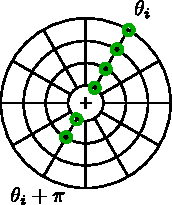
\includegraphics[width=0.5\textwidth]{fig/innerGhost}
    \caption{\textit{
The solid lines black lines represent the coordinate curves of a mesh with $4$ points in the $\rho$ direction (excluding the outermost ghost-point depicted with a dashed black line), and $8$ points in the $\theta$-direction.
The green solid circles represent the inner grid points at $\theta=\theta_i$, with the corresponding ghost-points at $\theta=\theta_i + \pi$ depicted as green dashed circles.
    }}
    \label{fig:innerRho}
\end{figure}
%
In this solution, the ghost-points for the innermost grid points in $\rho$ (those closest to the singularity) will be set to the value of the innermost grid point which lies $\theta + \pi$ away.
The next ghost-point will be set to the value of the second innermost internal point which lies $\theta + \pi$ away, and so on.
In this thesis, only one ghost-point is used.
With this method the second order FD stencil for the radial derivative becomes at the innermost point
%
\begin{align*}
    \L.\parti{f}{\rho}\R|_{\rho=\frac{\Delta \rho}{2}} \simeq
    \frac{-f\L(-\frac{\Delta \rho}{2}, \theta\R) + f\L(\frac{3\Delta \rho}{2}, \theta\R)}{2\Delta \rho}
    =
    \frac{-f\L(\frac{\Delta \rho}{2}, \theta+\pi\R) + f\L(\frac{3\Delta \rho}{2}, \theta\R)}{2\Delta \rho}.
\end{align*}
%
This method was used in \cite{Naulin2008}, and is shown to be second order accurate in \cref{sec:MES}.

\subsection{The inner boundary condition for \texorpdfstring{$\phi$}{the potential}}
\label{sec:innerPhiBC}
%
We also need an artificial ghost-point for the innermost point in $\rho$ for inversion method described in \cref{app:lapInv}.
As the inversion in the $\rho$ direction will be done for each mode, the method described in \cref{sec:ghostRhoDeriv} is not directly applicable.

Instead, we can set the inner ghost-point depending on the evenness of the mode.
If the mode is even, the mode under consideration would have the same value diametrically opposite of the innermost point.
Notice that this is true for every point at the same radius.
Hence, the ghost-point for the inner $\rho$ value is set to the same as the value at the innermost $\rho$.

If the mode is odd, the mode under consideration has different signs at diametrically opposite positions.
Thus, the ghost-point for the inner $\rho$ value is set to the negative of the value at the innermost $\rho$.
The method was first used in \cite{Naulin2008}, and is depicted in \cref{fig:BCLaplace}.
%
\begin{figure}[h!]
    \centering
    \begin{subfigure}[t]{0.5\textwidth}
        \centering
        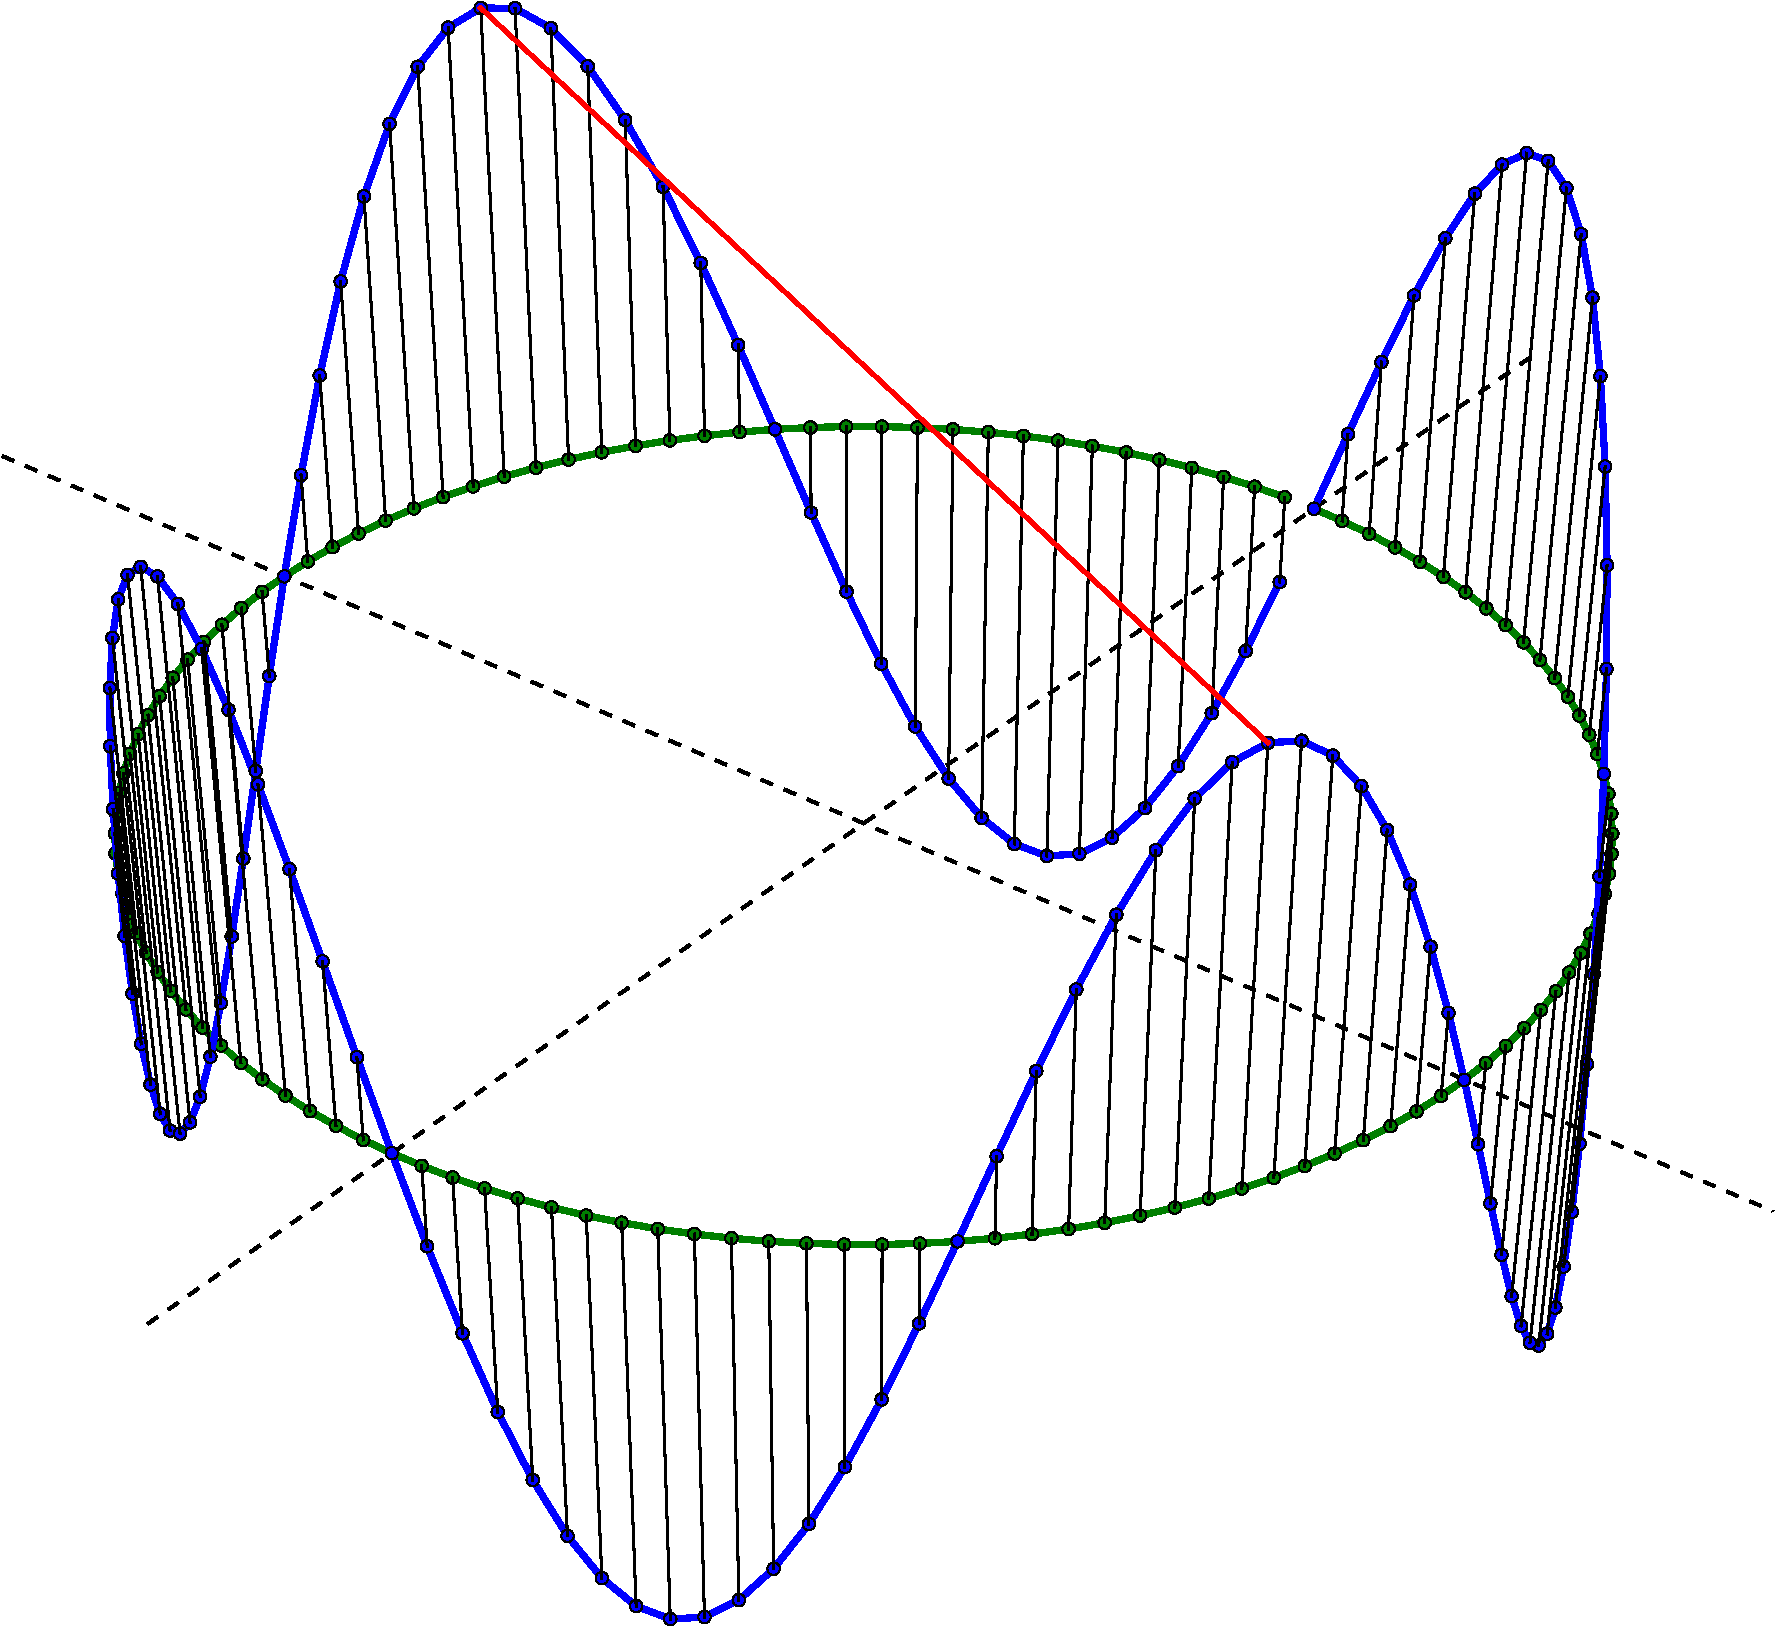
\includegraphics[width=0.8\textwidth]{fig/mode_4}
        \caption{An even mode.}
    \end{subfigure}%
    \hfill
    \begin{subfigure}[t]{0.5\textwidth}
        \centering
        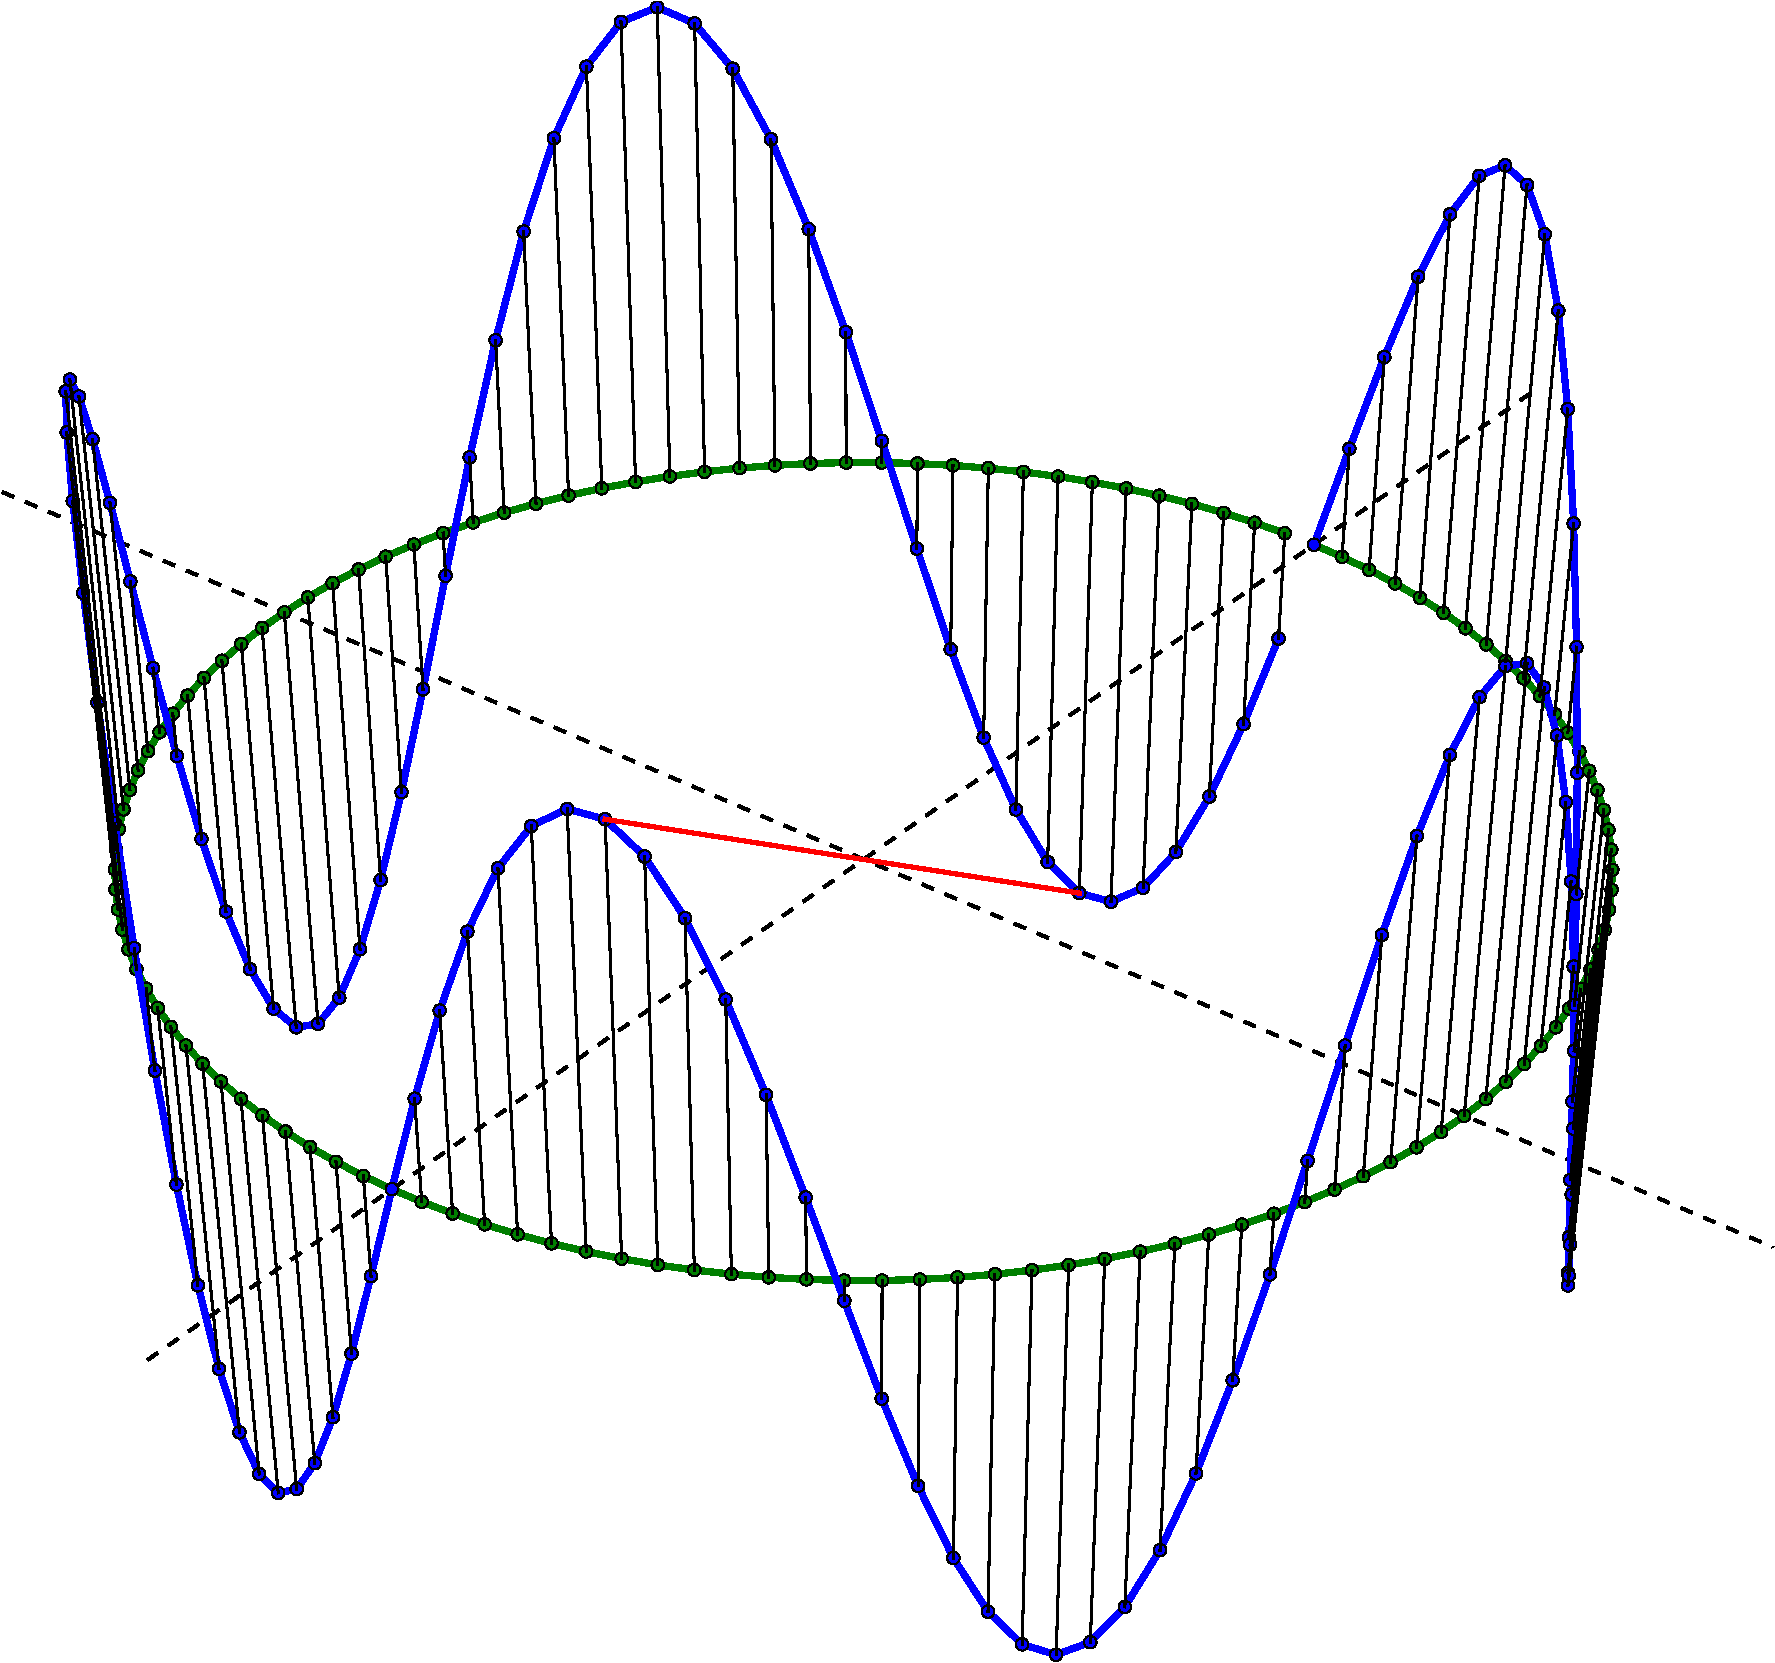
\includegraphics[width=0.8\textwidth]{fig/mode_5}
        \caption{An odd mode.}
    \end{subfigure}
    \caption{Two points diametrically opposite of each other has the same sign if the mode is even, but opposite signs if the mode is odd.
            The red solid line connects points diametrically opposite of each other.}
    \label{fig:BCLaplace}
\end{figure}
